\documentclass[10pt,twocolumn,letterpaper]{article}

\usepackage{cvpr}
\usepackage{times}
\usepackage{epsfig}
\usepackage{graphicx}
\usepackage{amsmath}
\usepackage{amssymb}
\usepackage{float}
\usepackage{caption}


% Include other packages here, before hyperref.

% If you comment hyperref and then uncomment it, you should delete
% egpaper.aux before re-running latex.  (Or just hit 'q' on the first latex
% run, let it finish, and you should be clear).
\usepackage[breaklinks=true,bookmarks=false]{hyperref}

\cvprfinalcopy 

\def\httilde{\mbox{\tt\raisebox{-.5ex}{\symbol{126}}}}


\graphicspath{ {images/} }


\setcounter{page}{1}
\begin{document}

%%%%%%%%% TITLE
\title{Spotting Distracted Drivers Using Classic CV Methods}

%%%%%%%%% Author Names
\author{Guillermo Reyes\\
{\tt\small enggreys@gmail.com}
\and
Daniel Schaefer\\
{\tt\small secondauthor@i2.org}
\and
Marc Tonsen\\
{\tt\small secondauthor@i2.org}
\and
Dominik Weber\\
{\tt\small secondauthor@i2.org}
}

\maketitle

%%%%%%%%% ABSTRACT
\begin{abstract}
   The ABSTRACT is to be in fully-justified italicized text, at the top
   of the left-hand column, below the author 
   information. Use the word ``Abstract'' as the title, in 12-point
   Times, boldface type, centered relative to the column, initially
   capitalized. The abstract is to be in 10-point, single-spaced type.
   Leave two blank lines after the Abstract, then begin the main text.
\end{abstract}

%%%%%%%%% BODY TEXT

\section{Introduction}


According to the U.S. Department of Transoprtation and National Highway Traffic Safety Administration, about 18\% of all injury crashes and 10\% of fatal crashes are reported to involve distracted drivers at the moment of the accident ~\cite{knuthwebsite}. In 2013 this, unfortunately, translated to over 3000 people killed and 400,000 people injured, in the United States alone due to motor vehicle crashes.

This clearly speaks for measures to be taken. Spotting distracted drivers in time could help to take appropriate actions and thus prevent accidents and save thousands of lives every year. In order to detect distracted drivers, different approaches have been taken. However, many of them are intrusive and expensive. However by using simple cameras combined with computer vision algorithms, one can get a solution that is both cheap and non-intrusive.\\

For this task we have entered the Kaggle Competition: State Farm Distracted Driver Detection ~\cite{Kaggle}. The challenge consists of classifying images of drivers engaging in the behaviors described below.

\begin{enumerate}
	\item Safe driving
	\item Texting with right hand
	\item Talking on the phone with right hand
	\item Texting with left hand
	\item Talking on the phone with left hand
	\item Operating the radio
	\item Drinking
	\item Reaching behind
	\item Hair and makeup
	\item Talking to passenger
\end{enumerate}

In this paper we propose different approaches to solve this task using some classic computer vision methods to find out how well they stack up against state of the art methods such Deep Neural Networks, which can already achieve up to 99\% accuracy .

% TODO erwaehnen von Computational Limits + allgemein gruende fuer die entscheidung kein cnn zu machcen


\section{Related Work}

There are already quite a few approaches regarding distracted driver distraction, although these approaches are mainly working on picture datasets with frontal-views on the face and rely almost exclusively on gaze-tracking or head-pose estimation. \cite{Dorazio} \cite{6957817}

Additionally some of these datasets are being captured in artificial environments (for example Racing Simulators) \cite{itsc:bergasa2008} which results in much more consistent variables like e.g. light situation and camera angle. In some of the approaches additional sensors are being used (e.g. RGB-depth cameras) which obviously also extend the possibilities greatly. \cite{Ragab2014}

We also decided to do some research on the very familiar topic ''Activity Recognition'' to explore further possibilities. Unfortunately most of the approaches in the Activity Recognition field rely on additional sensors (eg. wearable sensors) \cite{6258525} \cite{6365160} or rely on continious video instead of single pictures. \cite{1315249} \cite{1430826}

So our conclusion was that the current methods are not really applicable to the problems we wanted to solve, so we have to come up with something on our own!



\section{The Dataset}
The first step we took was analysing the dataset. We are given over 2.000 pictures per class from 26 different drivers in total. Each of the drivers has roughly the same amount of pictures per class. 

The drivers are split up in four cars. Depending on the car the camera angles varies. During the analysis process we also noticed that there is labeling noise in the data. For example we found several pictures in the ''safe driving'' class, which should in our opinion belong to the ''Talking to passenger'' one. Also lighting-conditions changed rapidly and the drivers have different ethnicities.


Additionally to this so called training set, of which we know the driver (and thus car) and class of each picture, we also have a so called test set containing around 80.000 unclassified pictures. The only option to verify results on this set is to upload them to the competition website, but because of the time necessary to classify all these 80.000 pictures combined with the fact that we only get very limited information back, we decided to run our tests only on parts of the training set to speed up our evaluation process.







\section{Proposed Methodology}


\subsection{Head-based classification}
\begin{figure}[h]
	\centering
	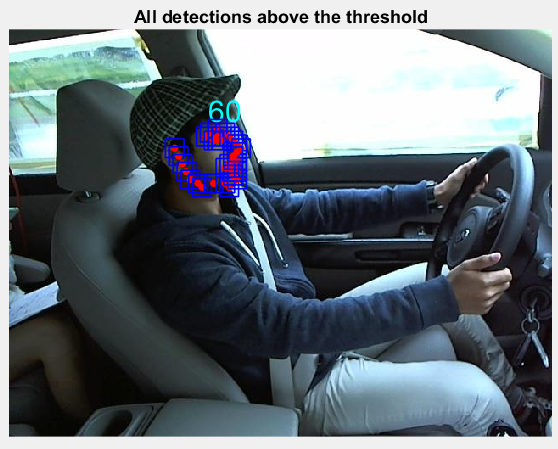
\includegraphics[width=0.2\textwidth]{face1}\hspace{0.01\textwidth}
	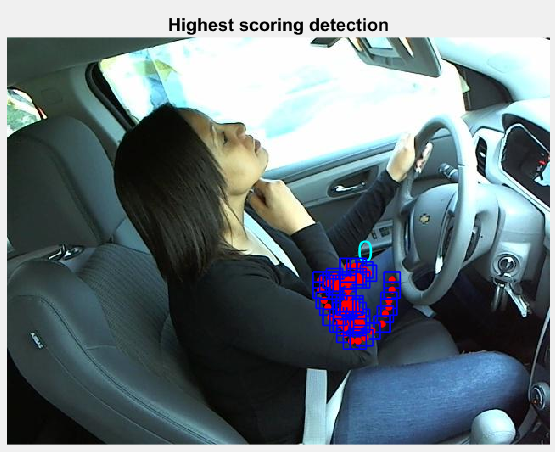
\includegraphics[width=0.2\textwidth]{faces/face7}\\ \vspace{0.01\textwidth}
	\caption{good and bad example of Face}
	\label{face_estimation_example}
\end{figure}
One of our ideas was to use a headdetector or a facedetector to extract a feature and predict the correct class or narrow down the possible classes. At least we hoped it would be possible to say if a picture is in a specific class or not. We tried about 7 different head or facedetecors and all had Problems to detect the head. We think the problem was that the pictures have a relative small resolution. An other Problem could be the different angles, because some detectors only worked with frontal view others only in the sideview. Long hair, sunglasses and other occlusion could be a problem too. In the end we found Face~\cite{Ramanan:2012:FDP:2354409.2355119}, which found heads in about 80\% of the pictures and gave us the horizontal angle from face to camera and 39 or 68 points of the face.Even if it found a face, it was not always the correct one. Face is runnning in matlab, so we used it to create a .csv file for every class + a file for the pictures where it was impossible to find a head. Then we let a Support Vector Machine and a Random learn on this data. First we only used the angle. Then we used angle and the points in relation to a fixed point in the face and hoped that these point could show us if the person is looking straight or lookung down on his mobilephone or the radio. We tried with both to predict the right class and to predict if the person is talking to the passenger or not.

\subsection{Hand-based classification}
\begin{figure}[h]
	\centering
	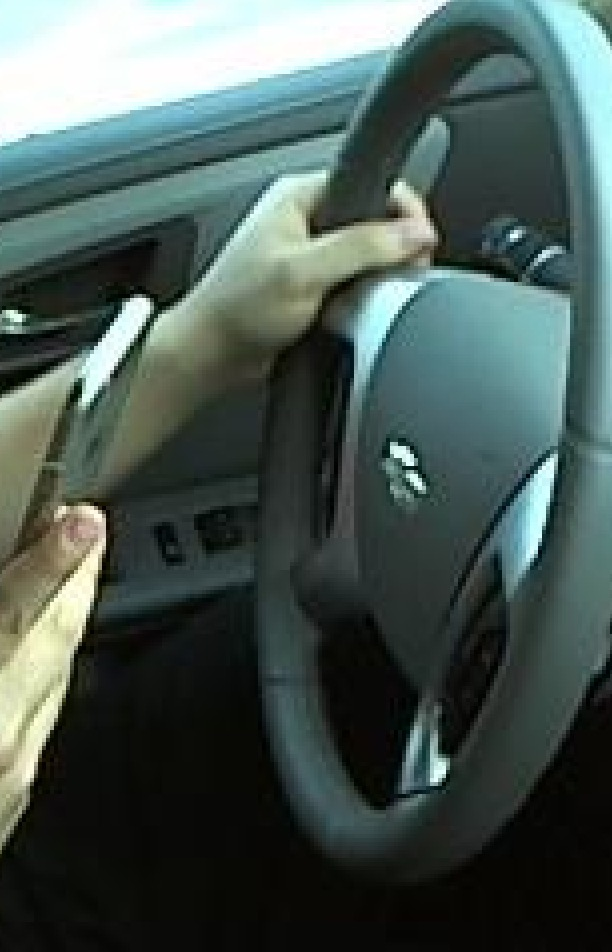
\includegraphics[width=0.2\textwidth]{handpose_example_1_cut}\hspace{0.01\textwidth}
	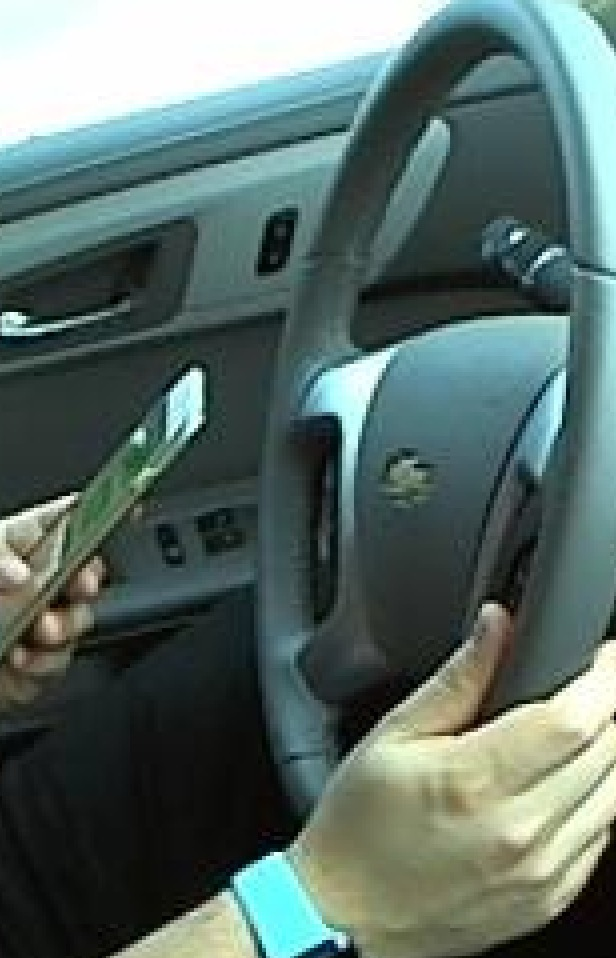
\includegraphics[width=0.2\textwidth]{handpose_example_2_cut}\\ \vspace{0.01\textwidth}
	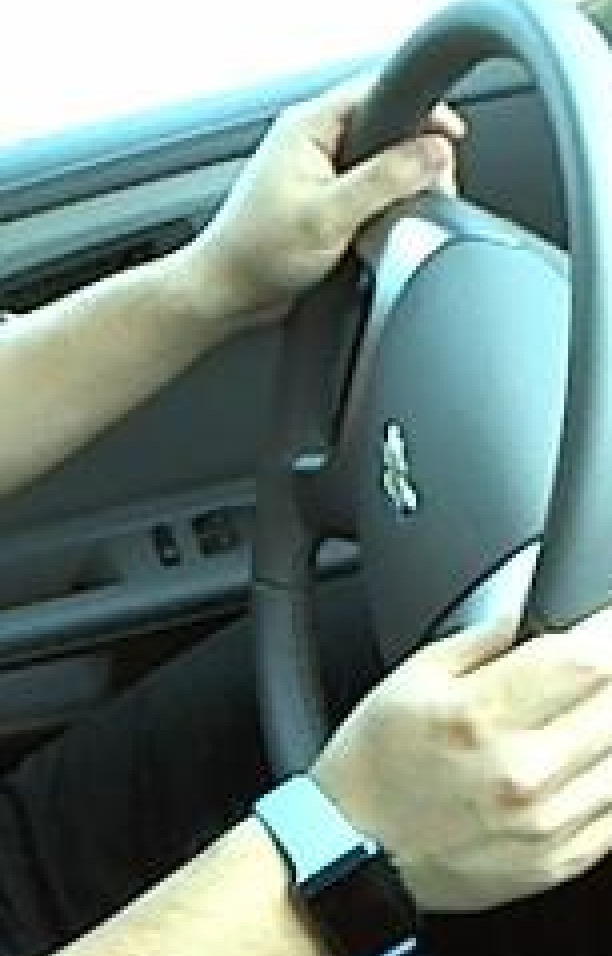
\includegraphics[width=0.2\textwidth]{handpose_example_3_cut}\hspace{0.01\textwidth}
	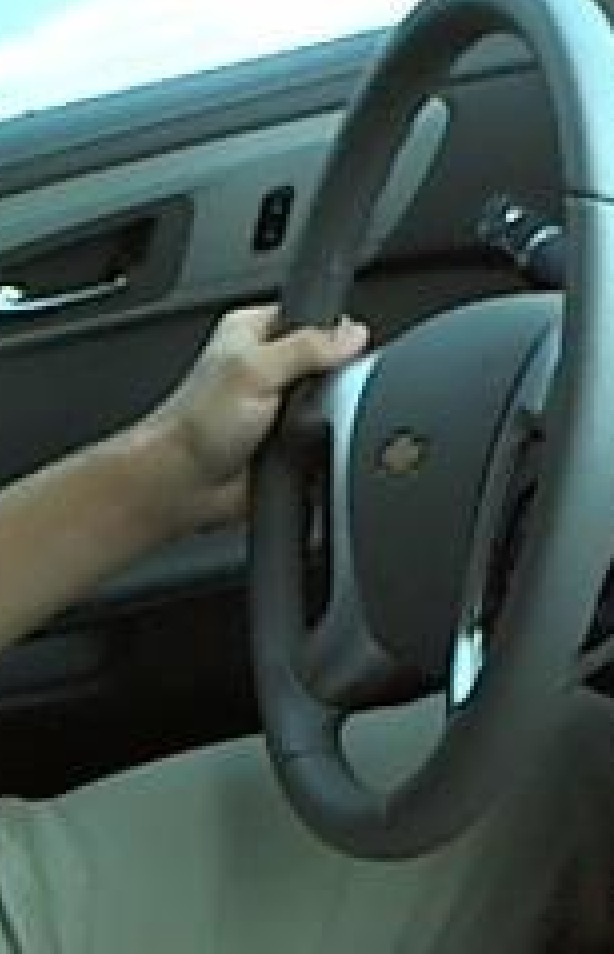
\includegraphics[width=0.2\textwidth]{handpose_example_4_cut}
	\caption{Examples of the cropped images we are using to train a classifier. The classes of the images from top-left to bottom-right are: Texting Right, Texting Left, Safe Driving, Reaching behind.}
	\label{hand_estimation_example}
\end{figure}
When examining the dataset, we found that many of the classes can be well distinguished when only considering the part of the image in the vicinity of the steering wheel. All of the activities described by the different classes in the task are performed with the arms, therefore their appearance is a strong indicator of the corresponding class. Based on this, we have cropped the images in the dataset to a fixed size of 155x240 px, to only contain the steering wheel and its immediate surroundings. See Fig. \ref{hand_estimation_example} for an illustration of those images and to see an example of how well some classes can be distinguished from that partial image. On those images we have trained a classifier to distinguish all classes and some to solve a 1-vs-1 classification task between only two classes. We have also tried to segment the classes into clusters and to classify based on those clusters, but our results were not satisfactory and we will not discuss this approach further. We have tried out different features for the classification:
\begin{itemize}
	\item \textbf{Raw Image}: We use a raw downscaled version of the image as a feature.
	\item \textbf{HoG}: Histogram of oriented gradients, which we have discussed in the lecture. We use the scikit-image implementation
	\item \textbf{LBP}: Local binary patterns, which is a feature originally developed for texture classification. It has been reported to work well in combination with HoG features in some cases. We also use the scikit-image implementation for this.
\end{itemize}
Besides using Support Vector Machines for classification, which was the only classifier discussed in the lecture, we have also tried Random Forrests.\\
It is important to note that the steering wheel is not aligned across the dataset. The training-data was recorded in 4 different cars with varying camera angles. As we will show, it is important to align the steering wheel in the cropped images for a good performance. We have manually labeled the center of all steering wheels to perform this alignment.


\subsection{Bodepose-based classification}
Its pretty obvious that reliable localisation of head and arms would easily allow us to differentiate almost all of the classes because of the different positions the mentioned body-parts are in, during the different distractions. On gitHub we found the open source implementation ''Convolutional Pose Machines'' which is able to predict the key bodyparts for us, like wrists, shoulders, elbows, neck and head. The paper was presented at the Conference on Computer Vision and Pattern Recognition in 2016 and outperformed everything else we found greatly using the pretrained models provided on gitHub. Unfortunately we could not use this implementation in our project, because of the computational performance neccessary. Nobody of us had access to a cuda-supported GPU with over 2GB of VRAM which was not nearly enough for this Pose-Machine to work. Doing everything on CPU was not an option for us because this took between 1-4minutes per picture. Although this at least made it possible to take a look at the results this pose machine is able to achieve. We can't really precisely evaluate the performance of this approach but in all the pictures we were able to test the heatmaps of the said body-parts are looking usable across all the different classes. You can see an example of how the heatmaps for interesting bodyparts look like in Figure \ref{BodyPoseExample}.\\
\begin{figure}[h]
    \centering
    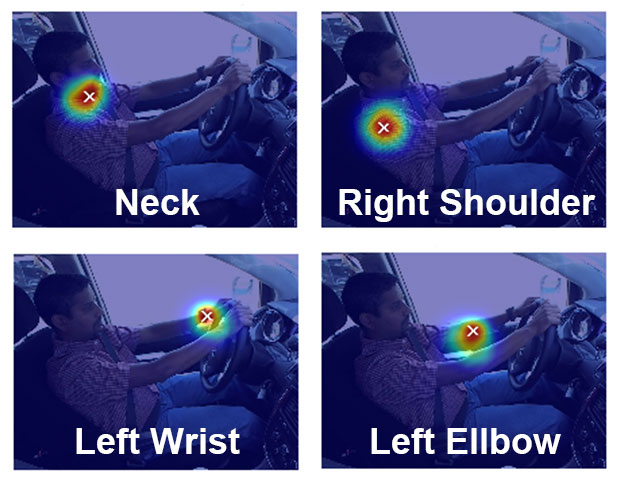
\includegraphics[width=0.5\textwidth]{BodyPoseExample}
    \caption{Example Heatmaps of Conbolutional Pose Machines}
    \label{BodyPoseExample}
\end{figure}

Without our computational limitations these bodypose-machines would probably be a very nice addition to the headpose and handpose estimation we are currently using.


\subsection{HOG Landmarks}
For the last approach used in this paper, we look for specific things in the images that help us make a decision. We call these specific things landmarks. A landmark can be anything in the images(pose, objects, etc.) that can be used to distinguish a class from the others. These landmarks are chosen arbitrarily in this paper and we shall later evaluate how well they perform. Below we outline what of these landmarks are, note that there is at least one distinctive landmark per class.

\begin{enumerate}
	\item Head facing front, towards the road.
	\item Head facing sideways towards the copilot
	\item Head facing backwards towards the back passengers.
	\item Empty gap in front of the head rest
	\item Right hand holding phone while texting
	\item Right hand holding phone while talking\
	\item Left hand holding phone while texting
	\item Left hand holding phone while talking
	\item Hand holding bottle/cup
	\item Hand near head
	\item Hand reaching behind
	\item Hand reaching for radio	
\end{enumerate}

In order to detect this landmarks, approximately 50 images per class were taken and manually labeled bounding boxes around the selected landmarks. The detectors were then trained based on HOG features for each landmark with the help of Dlib \cite{dlib09}.
After having trained the detectors, one can use these to determine whether a certain landmark is present in an image or not. Then, by training a simple SVC that uses as predictors an array of boolean features each one of which representing the presence, or absence, of a landmark, one can potentially predict the activity performed by the driver.



 



%\begin{minipage}[t]{.5\textwidth}
%	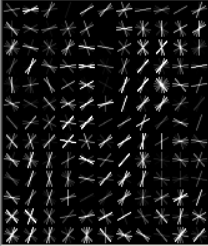
\includegraphics[width=\textwidth]{mult_HOG/HOG_phone}
%	\captionsetup{justification=raggedright, singlelinecheck=false}
%	\captionof{figure}{H Feistel Function}
%\end{minipage}%
%\begin{minipage}[t]{.5\textwidth}
%	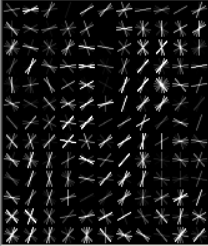
\includegraphics[width=\textwidth]{mult_HOG/HOG_phone}
%	\captionsetup{justification=raggedright, singlelinecheck=false}
%	\captionof{figure}{HOG of the right hand holding phone while texting landmark}
%\end{minipage}


%\begin{figure*}[h]
%	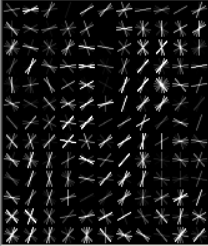
\includegraphics[width=0.85\columnwidth]{mult_HOG/HOG_phone}
%	\captionsetup{justification=raggedright,
%		singlelinecheck=false
%	}
%	\caption{HOG of the right hand holding phone while texting landmark}
%\end{figure*}





\section{Experimental Results}

\subsection{Hand-based classification}

	\subsubsection{Alignment of the steering wheel}
	\begin{table}
		\begin{tabular}{c|c|c|c}
			& Within 1 car & No alignment & With alignment \\ 
			\hline 
			Avg. Accuracy & 37\% & 10\% & 24\% \\ 
		\end{tabular} 
		\caption{Classification accuracies for different levels of steering wheel alignment.}
		\label{hand_estimation_alignment}
	\end{table}
	
	To investigate the impact of image alignment we have trained classifiers on 3 different sets of data:
	\begin{itemize}
		\item 11 participants recorded in the same car and with the same camera angle, who are therefore perfectly aligned
		\item Unaligned crops from all participants, i.e. a window with a fixed size and position
		\item Aligned crops from all participants based on our labellings of the steering wheel
	\end{itemize}
	As one can see in Table \ref{hand_estimation_alignment} alignment significantly improves the results. The results on data coming from only a single car can be regarded as an upper limit with 37\% accuracy. With no alignment the accuracy was only 10\% which is equal to random guessing, while the accuracy was 24\% with alignment. For all further experiments the steering wheels were therefore aligned.


	\subsubsection{Feature evaluation}
	\begin{table}
		\begin{tabular}{c|c|c|c|c}
			& Raw & HoG & LBP & HoG+LBP \\ 
			\hline 
			SVR & 25\% & 32\% & 23 \% & n.A. \\ 
			\hline 
			Random Forest & 27\% & 26\% & 16\% & n.A. \\ 
		\end{tabular} 
		\caption{Classification accuracies for different features and classifiers trained on 4 participant with 1 participant for testing.}
		\label{hand_estimation_features}
	\end{table}
	Consider the classification accuracies achieved by the different combinations of features and classifiers visible in Table \ref{hand_estimation_features}. They were computed for classifiers trained on the data of 4 participants and tested on 1 participant. By far the best result was achieved with an SVM and HoG features.
	
	\subsubsection{All vs All compared to 1 vs 1}
	\begin{figure}[h]
		\centering
		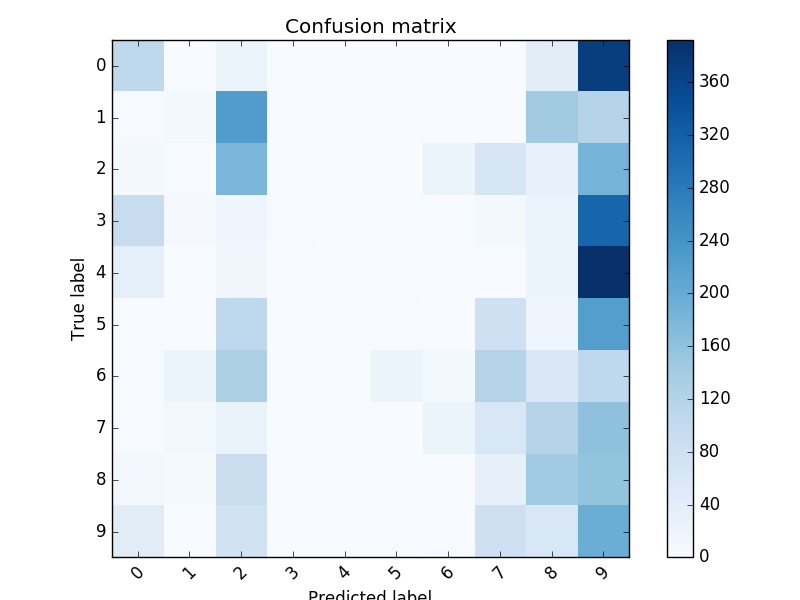
\includegraphics[width=0.5\textwidth]{handpose_plot_20p_c9}
		\caption{Confusion matrix for an SVM trained on HoG features of 20 participants (6 participants in test set).}
		\label{hand_estimation_cm}
	\end{figure}
	\begin{table}
		\begin{tabular}{c|c|c|c|c|c}
			& c1 vs c3 & c2 vs c4 & c0 vs c7 & c0 vs c5 & c3 vs c4 \\ 
			\hline 
			Accuracy & 98\% & 86\% & 94\% & 84\% & 91\% \\ 
		\end{tabular} 
		\caption{Classification accuracies for different 1-vs-1 classifiers trained on 8 participants (3 participants in test set).}
		\label{hand_estimation_1vs1}
	\end{table}
	Although the classification accuracy of an SVM with HoG features is significantly better then random with more then 30\%, it is not good enough to be practically relevant. The confusion matrix in Figure \ref{hand_estimation_cm} displays the classification errors of a classifier trained on 20 participants (6 participants in the test set) and HoG features. There does not seem to be any logically explainable confusion. To further investigate our thesis that some of the classes should be easy to distinguish based on the appearance of the hands on the steering wheel, we trained a few 1-vs-1 classifiers. As is illustrated in Table \ref{hand_estimation_1vs1}, they did achieve a very good accuracy. 
	
	
\subsection{HOG Landmarks}




\section{Conclusion}

\section{Future Work}



%%%%%%%%% REFERENCES

{\small
\bibliographystyle{ieee}
\bibliography{egbib}
}

\end{document}
